\mysection{User Interface Design}
In this section we will some mockups in order to describe Travlendar+ user navigation.

\mysubsection{Login \& User Profile}
The login interface is composed by email and password fields. After the insertion of the credentials the user will be able to access to his calendar and personal page.
\begin{figure}[H]
	\centering
	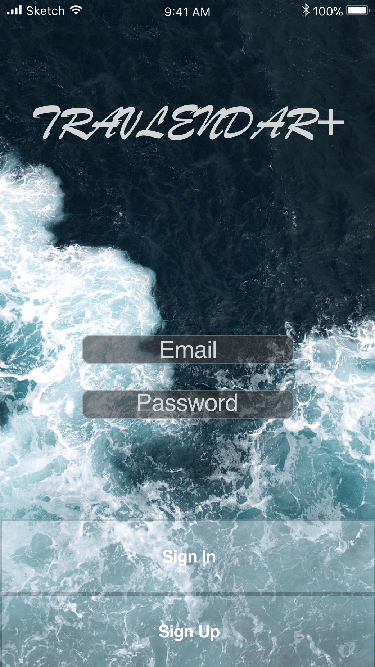
\includegraphics[scale=0.23]{Images/Interface/Login/1_login_form}
	\hspace{0.5cm}
	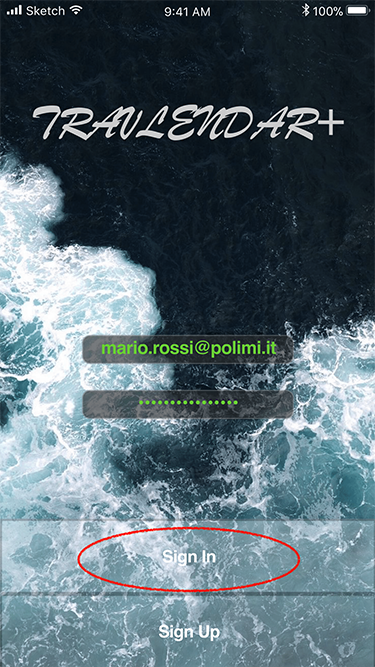
\includegraphics[scale=0.23]{Images/Interface/Login/2_login_form_filled}
	\hspace{0.5cm}
	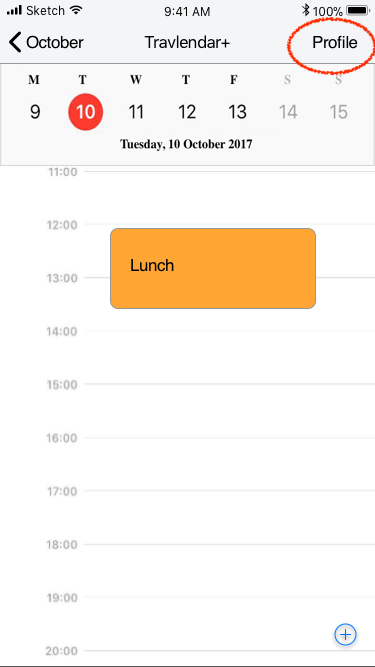
\includegraphics[scale=0.23]{Images/Interface/Login/3_calendar+lunch}
	\hspace{0.5cm}
	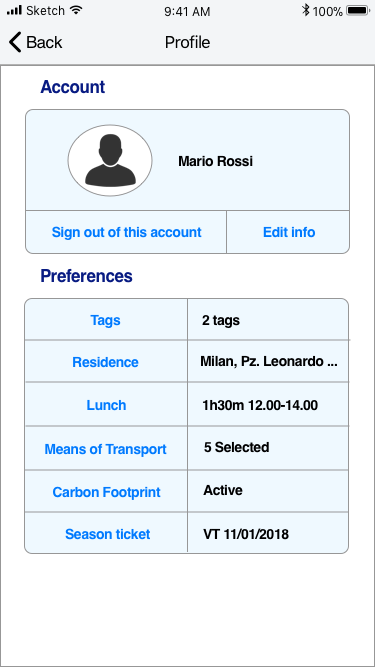
\includegraphics[scale=0.23]{Images/Interface/Login/4_profile_no_trips}
	\caption{Login Sketch}
\end{figure}

\mysubsection{Tags}
In this section the user can create tags by tapping on the add button set in the centre-bottom side of the UI.
The user is asked to assign a colour and a name to the tag.
\begin{figure}[H]
	\centering
	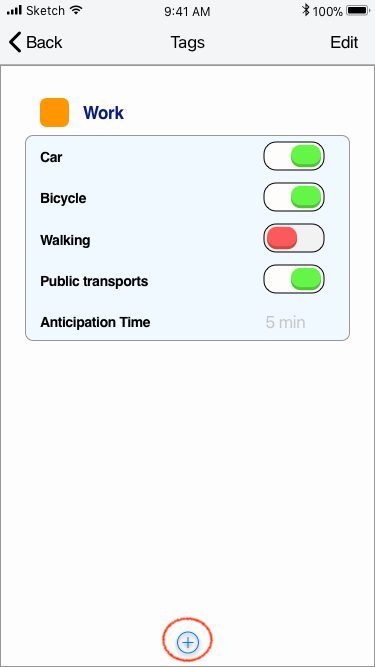
\includegraphics[scale=0.23]{Images/Interface/Tags/1_tags+work_add}
	\hspace{0.5cm}
	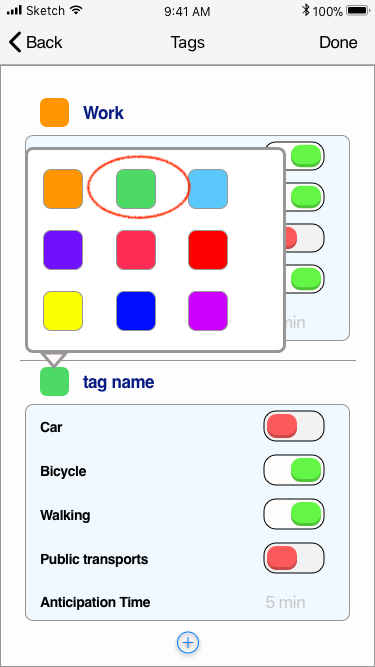
\includegraphics[scale=0.23]{Images/Interface/Tags/2_tags_color}
	\hspace{0.5cm}
	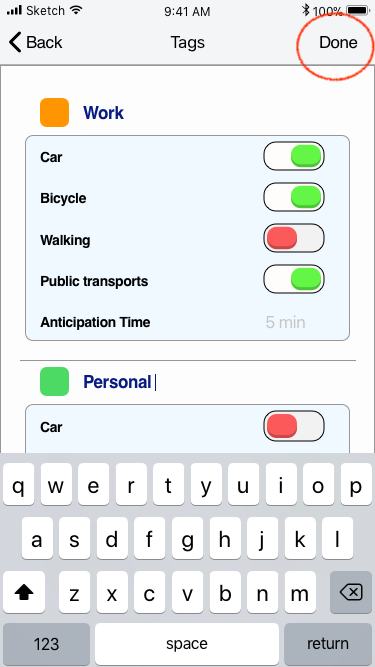
\includegraphics[scale=0.23]{Images/Interface/Tags/3_tag_name}
	\hspace{0.5cm}
	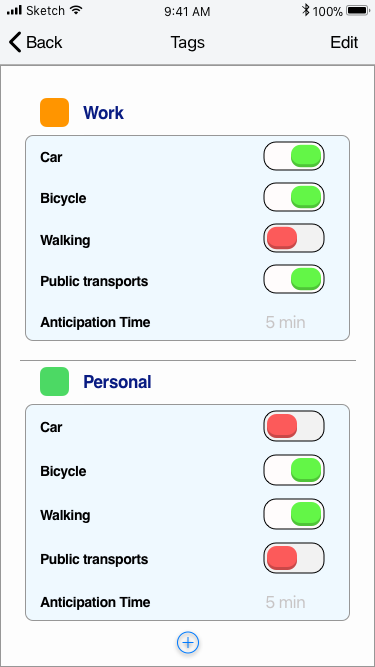
\includegraphics[scale=0.23]{Images/Interface/Tags/4_tags+work+personal}
	\caption{Add Tag Sketch}
\end{figure}
The user can delete one or more tag pressing on the “edit” and select the item he wants to delete.
\begin{figure}[H]
	\centering
	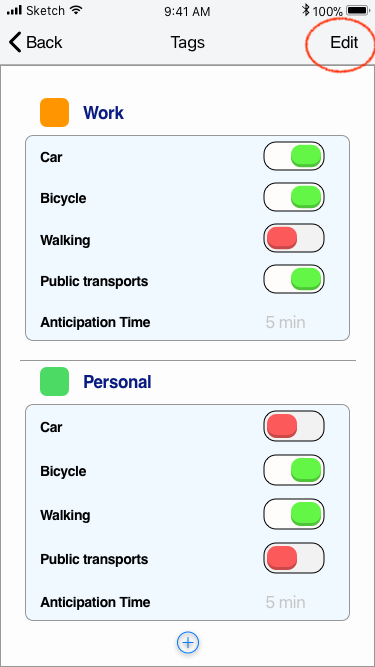
\includegraphics[scale=0.23]{Images/Interface/Tags/5_tags+work+personal-edit}
	\hspace{0.5cm}
	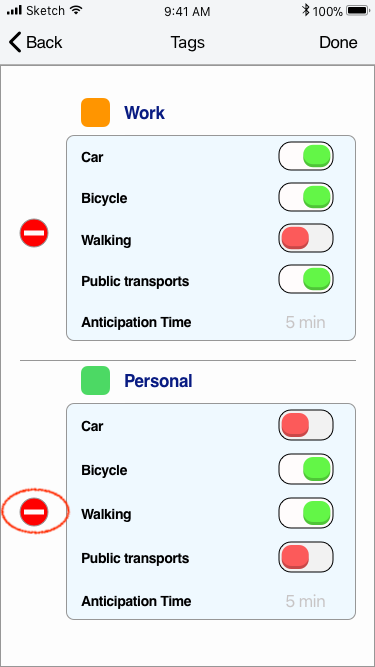
\includegraphics[scale=0.23]{Images/Interface/Tags/6_tags_deletion}
	\hspace{0.5cm}
	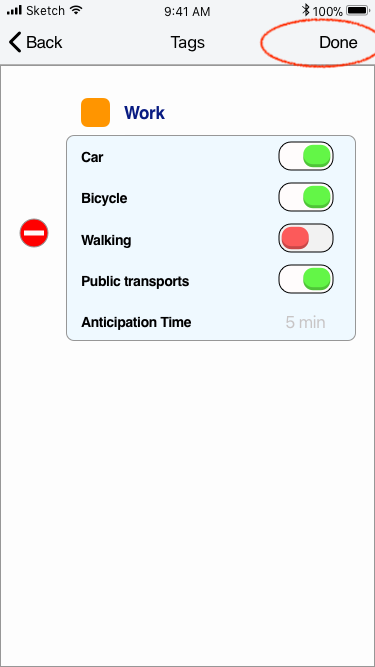
\includegraphics[scale=0.23]{Images/Interface/Tags/7_tags_deletion_2}
	\hspace{0.5cm}
	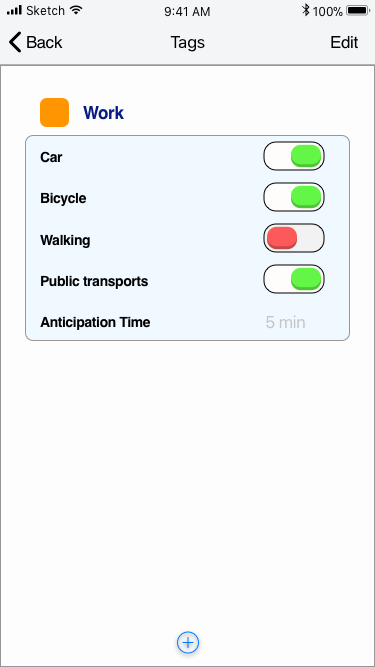
\includegraphics[scale=0.23]{Images/Interface/Tags/8_tags+work}
	\caption{Delete Tag Sketch}
\end{figure}